\documentclass[tikz,border=3mm]{standalone}
\usetikzlibrary{patterns}

\begin{document}
    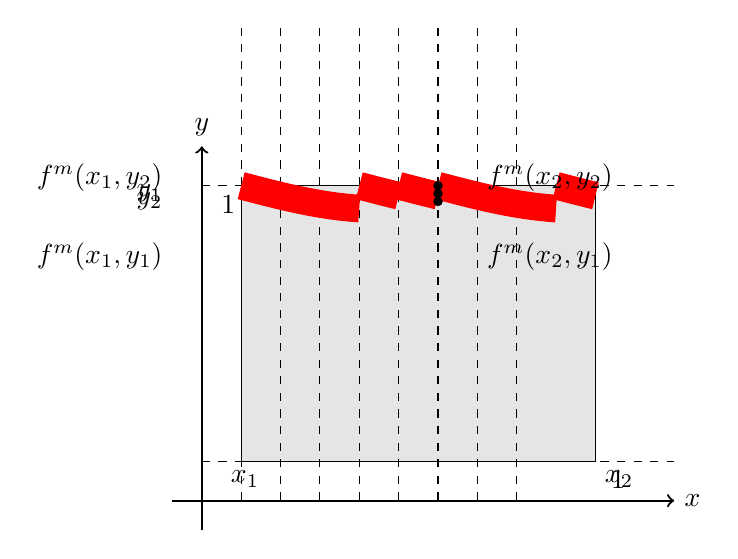
\begin{tikzpicture}[scale=0.5]
        % Axes
        \draw[thick,->] (-0.75,0) -- (12,0) node[right] {$x$};
        \draw[thick,->] (0,-0.75) -- (0,9) node[above] {$y$};
        
        % Unit box
        \draw[fill=black!10] (1,1) rectangle (10,8);
        
        % Dashed grid lines
        \draw[dashed] (0,1) -- (12,1);
        \draw[dashed] (0,8) -- (12,8);
        \foreach \y in {1,...,8}
            \draw[dashed] (\y,0) -- (\y,12);
        
        % Red regions
        \draw[red,line width=10pt,domain=1:4,smooth,samples=100] plot (\x,{8-0.6*sin(8*pi*(\x-1))});
        \draw[red,line width=10pt,domain=4:5,smooth,samples=100] plot (\x,{8-0.6*sin(8*pi*(\x-4))});
        \draw[red,line width=10pt,domain=5:6,smooth,samples=100] plot (\x,{8-0.6*sin(8*pi*(\x-5))});
        \draw[red,line width=10pt,domain=6:9,smooth,samples=100] plot (\x,{8-0.6*sin(8*pi*(\x-6))});
        \draw[red,line width=10pt,domain=9:10,smooth,samples=100] plot (\x,{8-0.6*sin(8*pi*(\x-9))});
        
        % Labels for the red regions
        \node at (7,8.2) [right] {$f^{m}(x_{2},y_{2})$};
        \node at (7,6.2) [right] {$f^{m}(x_{2},y_{1})$};
        \node at (-0.75,6.2) [left] {$f^{m}(x_{1},y_{1})$};
        \node at (-0.75,8.2) [left] {$f^{m}(x_{1},y_{2})$};
        
        % Points
        \filldraw[black] (6,7.6) circle (3pt);
        \filldraw[black] (6,7.8) circle (3pt);
        \filldraw[black] (6,8.0) circle (3pt);
        
        % Labels for x and y coordinates
        \node at (1.1,8) [below left] {$1$};
        \node at (11,1) [below left] {$1$};
        \node at (-0.75,7.6) [left] {$y_{2}$};
        \node at (-0.75,7.8) [left] {$y_{1}$};
        \node at (1.1,1) [below] {$x_{1}$};
        \node at (10.6,1) [below] {$x_{2}$};
    \end{tikzpicture}
\end{document}